La struttura alla base del mio tirocinio è facile da comprendere, ma allo stesso tempo non lo è stata la realizzazione di tutte le operazioni che si trovano dietro ad esso, in particolare il calcolo dello zoom ideale per rappresentare una determinata area geografica e il sistema alla base del movimento e caricamento delle tile aggiornate in base alle direzioni di spostamento. Analizzando la struttura del progetto, troviamo una pagina HTML contente una form con i dati di partenza per ottenere la mappa dell'area prescelta, un server che elabori le coordinate dei punti inseriti e ne ricavi lo zoom corretto e infine si occupi dello streaming dell'immagine corretta e infine l'interfaccia 3D, sviluppata utilizzando la libreria \textit{Three.js} con cui l'utente può interagire per ottenere le mappe in seguito allo spostamento in direzione nord, sud, est e ovest.

\section{Modellazione delle informazioni}
La prima sfida affrontata nel corso dello sviluppo del seguente progetto è stata sicuramente il modo in cui un utente volesse interfacciarsi con il sistema. Pensando a come, spesso, vengono consultate le mappe nei vari sistemi online, risulta macchinoso trovare, a partire da un centro ipotetico, il modo di visualizzare una determinata area. Proprio per questo motivo, si è preferito affrontare la problema dando la possibilià all'utente di inserire le coordinate dei vertici della zona d'interesse. Risulta a questo punto immediato il calcolo del centro. Infatti una volta inseriti i due punti il centro avrà come coordinate il punto medio delle due coordinate di partenza. Considerando dunque due punti a e b di coordinate $(lat_{a}, long_{a})$ e $(lat_{b}, long_{b})$ il centro corrispondente sarà:
\begin{center}

	\LARGE$(\frac{lat_{a}+lat_{b}}{2} , \frac{long_{a}+long_{b}}{2})$\par

\end{center}
Il passo in questo è stato abbastanza semplice, perchè essendo il centro di un sistema di riferimento bidimensionale in punto medio tra due punti è la media delle coordinate dei due punti. Affrontando però la questione dello zoom e dello spostamento, la soluzione non è stata altrettanto diretta e semplice, tanto che le questioni saranno affrontate in due paragrafi distinti.

\subsection{Il calcolo dello zoom adatto}
Il calcolo dello zoom è stato il primo problema affrontato nel corso dell'implementazione e della progettazione del progetto. Lo zoom nelle mappe di Google è un valore discreto che varia da 0 a 21 e per comprenderne il funzionamento è stato necessario capire cosa venisse rappresentato ad ogni livello. Nella proiezione adottata da Google al livello 0 l'intero globo viene raffigurato in un'immagine di 256x256 pixels di larghezze e altezza. Questo ha rappresentato un valore di riferimento per lo studio della funzione che calcoli lo zoom di partenza. Andando, infatti, ad analizzare sperimentalmente i successivi livelli di zoom ho visto che ponendo lo zoom a 1, 256 pixels erano diventati troppo pochi per rappresentare l'intero globo. A questo grado di zoom infatti sono necessari esattamente 512 pixels di larghezza e altezza per rappresentare l'intera immagine terrestre, esattamente il doppio. L'ipotesi, dunque, a questo punto formulata vuole che lo zoom non è altro che una progressione geometrica di ragione 2. L'ipotesi è stata successivamente verificata analizzando anche il terzo grado di zoom, nonostante non fosse possibile mostrare un'immagine di 1024 pixels per lato in quanto le API di Google limitano l'utilizzo delle mappe statiche a dimensioni di 640 pixel per lato. È, dunque, possibile riassumere lo zoom di Google con la seguente espressione: 
\begin{center}

	\large$256\times2^{zoom}$\par

\end{center}
Ad ogni livello, dunque, corrispondono un certo numero di pixel capaci di contenere la rappresentazione dell'intero globo, come è possibile vedere in tabella:

\begin{center}
\begin{tabular}{c @{\hspace{1em}} c}
Livello	& Pixels \\

0 & 256\\
1 & 512\\
2 & 1024\\
...	& ...\\
z & $256\time2^z$\\
... & ...\\
21 & 536.870.912\\

\end{tabular}
\end{center}

E' risultato a questo punto quasi immediato calcolare lo zoom necessario a rappresentare una determinata area geografica. Infatti, in 256 pixel sono contenuti tutti i 360 gradi della circonferenza terrestre, considerando che la nostra immagine sarà di 640 pixels la proporzione è già costruita:
\begin{center}

	\LARGE$\frac{640}{\Delta} = \frac{256}{360} $\par

\end{center}
Il $\Delta$ della nostra funzione sarà in questo caso la variazione di \textbf{longitudine} tra i due punti richiesti dall'utente. Una variante della stessa proporzione, andrà utilizzata per la latitudine, dove i gradi da rappresentare non sono 360, bensì 180, o meglio per rispettare la proiezione utilizzata da Google 170,1022, perchè i poli in questo tipo di rappresentazione vengono considerati come due punti approssimati all'infinito non saremo quindi in grado di vedere interamente tutti i 180 gradi di latitudine che vanno dal polo nord al polo sud, besì ne verranno raffigurati 85,0511 rispettivamente a nord e a sud dell'equatore.

A questo punto, una volta ottenuto il risultato del rapporto, è opportuno calcolare lo zoom, che come abbiamo visto può essere rappresentato come una potenza in base due. Dunque per passare dalla nostra proporzione al livello di zoom richiesto occorrerà eseguire il logaritmo in base due del risultato della proporzione:
\begin{center}

	\Large$log_{2}(\frac{640}{\Delta}\times\frac{360}{256}) $\par

\end{center}

Una volta ottenuto lo zoom necessario, a questo punto sarà sufficiente concatenare i valori del centro e dello zoom all'url di richiesta della mappa, fornito dalle API di Google\footnote{Vedi Capitolo 4, Paragrafo 2.3} per poter caricare la mappa richiesta.

\subsection{Calcolo dei centri successivi per lo spostamento}
Se per lo zoom, i ragionamenti e i calcoli sono stati immediati, o quanto meno molto lineari, la stessa cosa non si può dire del calcolo dei nuovi centri per aggiornare la mia mappa nello spostamento lungo la longitudine e, soprattutto, la latitudine.

Perchè dover calcolare un nuovo centro? All'apparenza può risultare abbastanza inutile o eccessivo doversi calcolare un nuovo centro ad ogni spostamento. Essendo centro e zoom i due attributi necessari per caricare una mappa, questa rappresenterà solamente un certo spazio angolare della terra in relazione anche alla dimensione dell'immagine che viene richiesta, sia per quanto riguarda la latitudine che per quanto riguarda la longitudine. Sarà, dunque, necessario una volta raggiunto un certo margine della mappa, caricare la mappa successiva e di conseguenza occorrerà ricavarsi il centro per richiederla. Il problema principale, però è legato alla proiezione che Google ha deciso di utilizzare per rappresentare la terra in piano. Come si sa, la terra non è piana ma una sfera leggermente schiacciata ai due poli. Proprio per questo motivo, non è possibile direttamente rappresentare la terra su di una immagine piana, senza aver fatto le dovute proiezioni. Diversi sono stati i teorici che hanno elaborato delle proiezioni cartografiche del pianeta, ma in particolare il nostro studio ha riguardato la \textbf{la proiezione cilindrica centrografica modificata di Mercatore}, creata dal matematico e astronomo Gerhard Kremer e utilizzata da Google nella variante della \textit{Web Mercator Projection}.

All'inizio, inconsapevolmente si erano trattate latitudine e longitudine in maniera indistinta, è stata dunque elaborata una semplice proporzione tra gradi e pixel, derivata da quella per il calcolo dello zoom, al fine di trovare il centro della mappa successiva, sia essa a nord, sud, est oppure ovest. Per il movimento longitudinale, dunque verso oriente e occidente, non sono emersi problemi. Riprendendo la proporzione precedente sappiamo che se a 360 gradi corrispondono a 256 pixels moltiplicati per la potenza in base 2 dello zoom, allora in 640 pixel ci saranno una certa quantità di gradi. Se sommiamo questa quantità alla longitudine del nostro centro, ne ricaveremo quella del centro successivo a oriente.
Ricostruendo la formula si ha che:
\begin{center}

	\large$ (\frac{640\times360}{256\times2^{zoom}}) + longitudine_{c} $\par

\end{center}
dove $longitudine_{c}$ è la longitudine del centro da cui ci stiamo movendo. 

In egual misura, se ci stiamo movendo verso occidente, sottraendo la stessa quantità alla longitudine del centro di partenza otterremo il nostro centro ad occidente:
\begin{center}

	\large$  longitudine_{c} - (\frac{640\times360}{256\times2^{zoom}}) $\par

\end{center}

Inizialmente, l'idea è stata applicata anche alla latitudine, muovendosi verso nord e verso sud. Ovviamente in questo caso la proporzione era stata modificata considerando i 170,1022 gradi complessivi dei paralleli terrestri. La funzione verrebbe così riprodotta:
\begin{center}

	\large$  latitudine_{c} \pm (\frac{640\times360}{256\times2^{zoom}}) $\par

\end{center}

I risultati inizialmente ottenuti non sono stati però quelli sperati. Il centro calcolato risultava sempre spostato, creando duplicazioni di alcune zone geografiche o a volte, addirittura, il completo taglio di altre. Dopo diversi fallimentari tentativi di approssimare il più possibile il calcolo, utilizzando, o teorizzando in alcuni casi, anche delle funzioni che in base alla latitudine approssimassero il punto in cui attaccare le mappe presenti sulla canvas. La risposta è stata trovata, alla fine, studiando la stessa proiezione di Mercatore.

Per la proiezione, un grado di latitudine all'equatore non vale quanto un grado di latitudine ai poli, questo è dovuto principalmente al diverso grado di distorsione presente in distinte aree geografiche della terra. Una rappresentazione di quanto appena detto può essere visto nell'immagine \ref{fig:mercatorproj}
\begin{figure}[H]
	\centering
	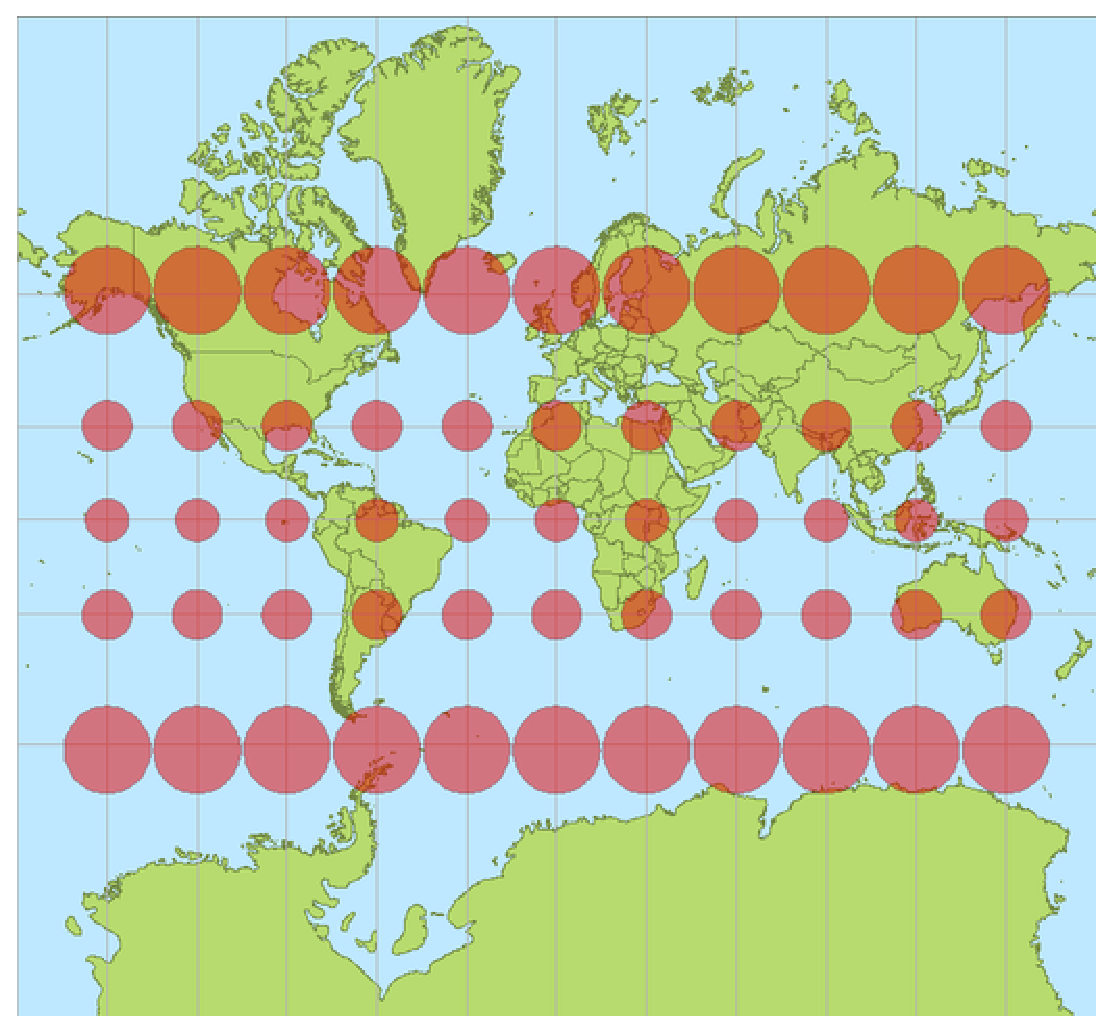
\includegraphics[scale=0.5]{figure/mercatorproj.eps}
	\caption{Rappresentazione della distorsione delle aree geografiche}\label{fig:mercatorproj}
\end{figure}

Seguendo questa proiezione, per effettuare i calcoli è stato necessario effettuare diverse conversioni. In primo luogo quella tra gradi decimali e radianti seguendo una semplice proporzione:
\begin{center}

	\Large$ \frac{deg}{180} = \frac{rad}{\pi} $\par

\end{center}

A questo punto è stato necessario applicare le conversioni forniteci dallo stesso Mercatore, per comprendere quale fosse il centro successivo a nord e a sud. 

Per prima cosa, è necessario passare dall'espressione in gradi a quella in radianti e successivamente occorrerà passare dal sistema di riferimento geoassiale al sistema in pixel utilizzando la seguente formula di conversione:
\begin{center}

	\Large$ \frac{1}{2}ln(\frac{1+\sin(lat)}{1-\sin(lat)}) $\par

\end{center}
dove $lat$ è la latitudine del nostro centro di partenza espressa in radianti. L'espressione riportata ha lo scopo di proiettare la latitudine dal sistema di riferimento geoassiale in un nuovo piano cartesiano. Bisogna dunque ragionare come se posizionassimo l'asse delle ordinate del nostro nuovo sistema lungo il meridiano zero o meridiano di Greenwich.

Una volta ottenuto questo valore, per ottenere la conversione del nostro punto sarà necessario aggiungerci la metà della dimensione del globo terrestre in pixel, secondo quella che è la dimensione di riferimento della proiezione, ovvero 256 pixels. Questo avviene perchè dovendo il nostro punto essere proiettato rispetto a quello che è il sistema standard, con la terra contenuta in una immagine quadrata di lato 256 pixels. La posizione del centro nel piano geoassiale, con coordinate (0,0), sarà sicuramente nella posizione $ (\frac{256}{2}, \frac{256}{2})$, dovremo dunque tener conto di questo valore nella nostra trasformazione. L'espressione riassunta è la seguente:
\begin{center}

	\large$ \frac{256}{2} + \frac{1}{2}ln(\frac{1+\sin(lat)}{1-\sin(lat)}) $\par

\end{center}

Ottenuta questa trasformazione, per ottenere la posizione del nuovo centro occorre considerare altri due valori caratterizzanti per ogni tipo di mappa, il livello di zoom e la dimensione in pixels. Infatti una volta ottenuto il valore di proiezione con la formula data sarà sufficiente sommare o sottrarre la metà dell'altezza della mappa fratto la potenza in base due dello zoom, per ottenere rispettivamente il centro a sud e a nord della nuova mappa, come riportato nella seguente formula:
\begin{center}

	\large $ lat_{px} \pm \frac{\frac{h}{2}}{2^{zoom}} $\par

\end{center}
con $lat_{px}$ il valore della latitudine convertito in pixels e h l'altezza della nostra figura.

Una volta ottenuto questo valore, sarà necessario effettuare una controinversione che riporterà il riferimento nelle coordinate terrestri, così da essere concatenate poi all'url di richiesta.
La formula inversa della conversione è la seguente:
\begin{center}

	\large $2tan^{-1}(e^{\frac{y-128}{\frac{-256}{2\pi}}}) - \frac{\pi}{2}$\par

\end{center}
Una volta convertito il valore da radianti in gradi sarà possibile utilizzare il risultato nella nostro sistema di movimento.

\section{Il processamento dei dati e la richiesta della mappa}
Avendo capito la proiezione e aver ricavato tutti i dati necessari dalla mappa, a questo punto sarà possibile creare il nostro sistema. Il servizio da me creato all'avvio mostra una semplice interfaccia grafica con una form che permette all'utente di inserire i dati dell'area geografica inizialmente richiesta:
\begin{lstlisting}
<form action="/map" method="post">
    North<br>
    Lat : <input type="text" name="n_lat"><br>
    Lon: <input  type="text" name="n_long"><br>
    <br>
    South<br>
    Lat : <input type="text" name="s_lat"><br>
    Lon: <input type="text" name="s_long"><br>
    <button type="submit">Submit</button>
</form>
\end{lstlisting}
Come si può evincere, l'utente può inserire i valori di latitudine e longitudine di due punti, uno a nord e l'altro a sud che rappresenteranno gli angoli della mappa visualizzata. Non viene specificato se Nord-est, Nord-ovest o Sud-est, Sud-ovest in quanto non cambia ai fini del calcolo delle distanze angolari tra i due punti. Come si può notare dagli attributi del tag \textit{form} nella porzione di codice sopra riportata il tasto "submit" della form, evoca un metodo post nel server, che si attiverà ed inizierà il processamento dei dati.

In particolare il metodo, richiamato dal percorso "/map", prende i dati dell'input, ne estrapola lo zoom, la dimensione esatta dell'area in pixel e le coordinate del centro e le invia sotto forma di pacchetto json al client. Nella porzione di codice possiamo vedere l'implementazione del metodo.
\begin{verbatim}
router.post("/map", function (req, res){
    var n_lat = parseFloat(req.body.n_lat);
    var n_long = parseFloat(req.body.n_long);
    var s_lat = parseFloat(req.body.s_lat);
    var s_long = parseFloat(req.body.s_long);

    var zoom = Math.min(zoom_lat(Math.abs(n_lat- s_lat)),
        zoom_lon(Math.abs(n_long - s_long)))+1;
    var c_lat = (n_lat+s_lat)/2;
    var c_lon = (n_long+s_long)/2;
    var h = height(Math.abs(n_lat - s_lat),zoom);
    var w = width(Math.abs(n_long - s_long), zoom);
    var a = req.body;
    a.zoom = zoom;
    a.c_lat = c_lat;
    a.c_lon = c_lon;
    a.height = h;
    a.width = w;
    res.render("map", a);
});
\end{verbatim}
Come è possibile notare vengono richiamati all'interno del metodo altri algoritmi, oltre a quello dello zoom, calcolato per la latitudine e per la longitudine e di cui poi viene ritornato il valore minimo, troviamo anche i metodi che calcolano le dimensioni in pixel della nostra area geografica. Infatti, anche se la mappa da noi richiesta è una mappa di dimensioni 640x640, la scelta è di mostrare solamente una porzione di essa, quella i cui margini sono definiti dai punti richiesti dall'utente.

Di seguito possiamo vedere il codice dei due metodi:
\begin{verbatim}
var height = function(d,z){
    var altezza = (256*Math.pow(2,z)*d)/latitude;
    return altezza*0.7;
};

var width = function(d, z){
    var larghezza = (256*Math.pow(2,z)*d)/longitude;
    return larghezza;
}
\end{verbatim}
Come si può notare l'altezza è stata adattata moltiplicandola per un fattore di 0.7, questo è dovuto allo stesso problema di cui si è trattato nel paragrafo 4.1.2. Infatti, questo valore moltiplicativo consente di approssimare il più possibile il risultato senza tagli anomali, che essi siano troppo grandi o troppo piccoli, per quanto riguarda invece la larghezza, come avviene per il calcolo della longitudine essa non ha mostrato problemi risultando invece in linea con la proporzione utilizzata. I due valori di "Latitude" e "Longitude" sono rispettivamente 170.1022 e 360, ovvero i gradi complessivi della latitudine e longitudine terrestre.

Una volta dunque ottenuti tutti questi parametri, è possibile creare il flusso streaming della mappa. Per la realizzazione di questo metodo mi sono affidato alla funzione "pipe" presente in \textit{Node.js}. La funzione è stata implementata nel seguente modo: 
\begin{verbatim}
router.get('/image/:c_lat/:c_lon/:zoom', function(req, res) {
    var url = 'https://maps.googleapis.com/maps/api/staticmap?size='+
    	'640x640&key=YOUR_API_KEY&center=';

    request(url+req.params.c_lat+","+
    	req.params.c_lon+"&zoom="+req.params.zoom).pipe(res);
});
\end{verbatim}
Attraverso questo metodo avviene dunque il caricamento della mappa che rappresenterà la texture degli oggetti sulla nostra scena 3D, che andremo ora ad analizzare nel dettaglio.

\section{Proiezione nella vista prospettica, il client Three.js}
Ho analizzato precedentemente come impostare la scena Three.js e, naturalmente, anche il progetto di questo "navigatore" seguirà lo stesso schema. Pur mantenendo la stessa struttura, il mio script avrà, come è normale, al suo interno diverse variabili in più oltre a quelle che abbiamo visto nel paragrafo introduttivo a questa tecnologia\footnote{Vedi paragrafo 2.2.1}. Evitando di trattare nuovamente di tutte le caratteristiche ambientali da dichiarare e come dichiararle, la concentrazione sarà rivolta direttamente alle componenti importanti del progetto.

Il primo elemento di cui mi trovo a parlare è il piano su cui posizionare la mappa come texture. Andando per gradi, analizziamo la struttura del codice:
\begin{verbatim}
var geometry = new THREE.BoxGeometry(640,640,0.1);
var plane;
var c_lon, c_lat;
var z = parseFloat("<%=zoom%>")
...
function init(){
	c_lon = parseFloat("<%=c_lon%>");
    c_lat = parseFloat("<%=c_lat%>");

    texture = THREE.ImageUtils.loadTexture("/image/"+c_lat+"/"+
    	c_lon +"/"+z, {}, function () {});
    texture.minFilter = THREE.LinearFilter;
    material = new THREE.MeshBasicMaterial({ map: texture, 
    	color: 0xffffff});
    plane = new THREE.Mesh(geometry, material);
    plane.rotation.x=-Math.Pi/2
    scene.add(plane);
    ...
}
\end{verbatim}
La prima cosa che si analizza da questa porzione di codice è l'aver dichiarato una variabile geometry che definisce la struttura di semplice scatola piatta (una altezza di 0.1) e di forma quadrata con lato 640. Questa sarà la geometria che ricorrerà per ogni piano che verrà creato o inizializzato durante lo spostamento, azione che successivamente analizzerò nel dettaglio. Un'altra cosa che si nota è che i due centri una volta dichiarati, vengono concatenati nel path di richiesta dell'immagine, che richiama il metodo di streaming presente nell'architettura del codice di back end. Infatti, il metodo presente nella package THREE.ImageUtils, loadTexture, viene utilizzato per caricare la texture da una fonte locale. In questo caso la fonte non è locale ma remota, il tutto è semplicemente superato dallo streaming del flusso di dati, che permette al client di caricare e renderizzare sul piano la mappa. La texture viene caricata come elemento del materiale attraverso l'attributo "map". Infine prima di essere aggiunto alla scena, il piano viene ruotato di 90 gradi per permettere la sua perfetta visualizzazione, in una prospettiva di 45 gradi.

Mancano ancora, però, alcuni dettagli di cui avevo parlato precedentemente, ovvero i due valori di "height" e "width". Come detto precedentemente, la mappa che abbiamo trovato, non sarà grande precisamente quanto l'area richiesta, bensì più grande. Proprio per questo motivo avevamo introdotto i valori di altezza e larghezza. Three.js, non ha una funzione che permetta il taglio di oggetti o di mostrare solamente una parte di essi. Dal momento in cui avevo bisogno di realizzare una struttura simile, ho iniziato alle diverse soluzioni da approcciare per la realizzazione del problema che si era creato. Come dicevo nella descrizione di questa libreria, una delle caratteristiche principali è sicuramente la sua licenza libera e open source. Proprio per questo motivo moltissimi sviluppatori nel web hanno implementato, e stanno implementando, librerie complementari al framework di Mr.doob. Una di queste è la libreria \textbf{csg.js}, completamente gratuita e disponibile su Github tra le repositories del suo ideatore Evan Wallace\cite{git:csg}. Questa libreria permette di costruire oggetti compositi. Infatti lo stesso nome è l'acronimo di Constructive Solid Geometry. Grazie a questa libreria ho creato un nuovo piano posizionato al di sopra del piano della mappa, e che oscura tutto il contenuto della mappa al di fuori dell'area d'interesse richiesta dall'utente. Un'applicazione della libreria può essere visto in questo esempio:
\begin{verbatim}
var aux = new THREE.BoxGeometry("<%=width%>", 
	"<%=height%>", 0.1);
var auxMesh = new THREE.Mesh(aux);
var auxBSP = new ThreeBSP(auxMesh);

var logical = new THREE.BoxGeometry(20000, 20000, 0.1);
var logicalMesh = new THREE.Mesh(logical);
var logicalBSP = new ThreeBSP(logicalMesh);

var newPlaneBSP = logicalBSP.subtract(auxBSP);
var newMaterial = new THREE.MeshBasicMaterial(
	{color: 0xffffff});
auxPlane = newPlaneBSP.toMesh(newMaterial);
auxPlane.position.y = 0.6;
auxPlane.rotation.x = -Math.PI/2;

scene.add(auxPlane);
\end{verbatim}
Gli oggetti vengono prima inizializzati come "mesh" per essere introdotti nella scena Three.js, successivamente convertiti in BSP, come richiesto dalla libreria di supporto e infine in seguito all'operazione di combinazione, in particolare la sottrazione dei due piani per poter ottenere un piano forato delle dimensioni richieste, si ha l'ultima conversione in mesh per essere aggiunto alla scena. Il piano risulterà ruotato di 90 gradi e rialzato su y di 0.6 pixel per evitare contatti tra i piani che ne compromettano la visualizzazione durante gli spostamenti.

Una volta impostata la scena, non ci resta che parlare nel dettaglio delle due azioni che l'utente potrà effettuare sulla mappa.

\subsection{Il sistema di movimento}
Affinchè il progetto risultasse interattivo e funzionale, occorreva rendere dinamica l'interazione con l'utente, volendo ricreare quelle che sono di fatto le dinamiche base offerte dai diversi sistemi di navigazione su mappa presenti nel web. Uno di questi è senza dubbio la possibilità di spostarsi sulla stessa mappa, una volta caricata la tile di riferimento. Per questo scopo, si è deciso di implementare un sistema di movimento che necessita l'uso dei soli tasti freccia della tastiera.

Three.js non possiede al suo interno delle funzioni che catturino l'utilizzo da parte dell'utente della tatiera, è stato dunque necessario far riferimento ad una nuova libreria di supporto, anch'essa sviluppata a partire dalla libreria base estendendo ulteriolmente le funzionalità della stessa. Mi sto riferendo alla libreria \textbf{THREEx}, una estensione di Three.js, rivolta principalmente allo sviluppo di videogames. Grazie a questo framework è stato possibile catturare lo stato della tastiera. Per utilizzarla, a tal scopo, è stato sufficiente dichiarare all'inizio del nostro script una variabile \textit{keyboard} in questo modo:
\begin{verbatim}
var keyboard = new THREEx.KeyboardState();
\end{verbatim}
La funzione \textit{KeyboardState()} permette di monitorare in tempo reale lo stato della tastiera, nel momento in cui premeremo un tasto esso attiverà un evento, principalmente booleano che ci permetterà di interagire con la mappa.

I tasti da noi monitorati per il progetto sono 6:
\begin{itemize}
	\item Tasti freccia (su, giù, destra e sinistra) per lo spostamento lungo gli assi geografici;
	\item Tasti W e S per lo zoom in e zoom out (di cui parlerò nel prossimo paragrafo).
\end{itemize}

Analizzando nel dettaglio la struttura del sistema di movimento per prima cosa è necessario definire una nuova funzione alla struttura del nostro script: la funzione \textit{update()}. Questa funzione verrà richiamata subito dopo il metodo render(), presente nella funzione animate() del nostro progetto Three.js.

Non volendo mostrare dettagliatamente il movimento per ogni lato, prenderò come riferimento il modello dello spostamento a nord rispetto alla nostra area di partenza. Il problema che mi sono inizialmente posto è stato quello del voler ottenere un movimento che fosse il più fluido possibile, rappresentando la maggiore area che sia possibile. Soprattutto, per rendere il movimento fluido, occorre caricare le nuove mappe, prima che la nostra area visualizzata ecceda la dimensione dell'immagine di partenza, e che soprattutto questa operazione venga applicata ciclicamente alla fine di ogni tile. Per questo motivo ho creato un ciclo while che prenda come riferimento la posizione del nostro oggetto plane lungo l'asse su cui si sta spostando, dunque l'asse X o Z. La posizione del piano verrà confrontata con le dimensioni della nostra area di visualizzazione, i parametri \textit{width} e \textit{height} che avevamo definito precedentemente lato server, che ci aiuteranno a ricavare la posizione di controllo. Infatti avendo un quadrato di 640 pixel per lato come immagine, sappiamo che la dimensione dell'area nascosta della nostra mappa precaricatà sarà:
\begin{center}
	\Large$\frac{640 - h}{2}$\par
\end{center}
A questo punto la condizione del nostro ciclo while è presto costruita:
\begin{verbatim}
while(plane.position.z > ((640 - h)/2))
\end{verbatim}

Per visualizzare l'area più grande disponibile, si è deciso di non raffigurare solamente il piano sequenzialmente attaccato, ma bensì 3 nuovi piani, che rappresenteranno nel nostro caso, lo spostamento a nord, le aree a nord, nord est e nord ovest. Per evitare comunque la sovrapposizione di troppe immagini che potrebbe causare un rallentamento nella fluidità del movimento, oltre che un glitch grafico nella rappresentazione, si aggiungeranno alla scena solamente i piani a nord est e nord ovest, poichè le due metà adiacenti degli stessi compongono la stessa area rappresentata dall'immagine a nord. A questo punto come nello scorrimento di una lista vengono aggiornati i riferimenti ponendo il piano di partenza come piano inferiore e il nuovo piano non aggiunto come piano di riferimento per proseguire lo spostamento, in questo modo sarà possibile al verificarsi nuovamente della condizione del ciclo while caricare i nuovi piani successivi. Una volta aggiunti i piani e aggiornati i riferimenti, i vecchi piani ormai lontani dal centro della nostra visualizzazione vengono eliminati dalla scena per alleggerire il carico grafico del progetto.

Si può vedere un esempio dell'algoritmo implementato, omettendo la definizione dei nuovi piani poichè uguale a quella fatta per l'oggetto di partenza: 
\begin{verbatim}
funtion update(){
	var moveDistance = 1;
	if ( keyboard.pressed("up") ){
	    newClat = getNorth(c_lat, z, 640);
	    cEs = eastCenter(c_lon);
	    cWe = westCenter(c_lon);
	    plane.position.z += moveDistance;
	    while(plane.position.z > ((640 - h)/2)){
            c_lat=newC_lat;
            scene.remove(supPlane, supE, supW);
            scene.add(plane);
            ...
            scene.add(supW, supE);
            scene.remove(infPlane, infE, infW);
            infPlane=plane;
            plane=supPlane;
            infE=supE;
            infW=supW;
            supE=null;
            supW=null;
            supPlane=null;
}
\end{verbatim}
Come visto nel paragrafo sulla modellazione delle informazioni, al fine di calcolare le nuove coordinate geoassiali, vengono calcolati i nuovi punti di riferimento, nel nostro caso sono a nord, nord est e nord ovest, e proprio per questo le variabili newClat, cEs e cWe rappresentano ripettivamente: la latitudine dei centri a nord, la longitudine del centro nord est e quella del punto a nord ovest.

Al pari del movimento a nord, la stessa tipologia di algoritmo è stato implementato a sud, a ovest e a est, cambiando naturalmente i riferimenti in base al verso dello spostamento.

Le mappe verranno caricate come effettuato nella creazione della scena, richiamando il server per lo streaming dell'immagine.

\subsection{Il sistema di zoom}
Al pari del sistema di movimento anche per lo zoom va fatta una menzione speciale. Infatti anche in questo caso, il ragionamento è molto simile, seppur riferendosi in questo caso ad uno spostamento sull'asse delle Y. Lo spostamento in questo caso è solamente utilizzato per ricreare un effetto di avvicinamento o allontanamento dall'area in cui ci troviamo. Come introdotto precedentemente, i tasti utilizzati in questo caso sono W ed S, rispettivamente per lo zoom in e zoom out. L'effetto dello zoom, cambierà ovviamente l'area visualizzata e aumenterà o diminuirà i dettagli su di essa visibili.

Anche in questo caso come per il movimento si effettua un controllo su un valore prefissato muovendo i piani di un valore pari a 0.2 lungo l'asse Y, fino al raggiungimento del valore di 7. In quel momento, verrà caricato un nuovo piano, denominato zoomP, con la mappa centrata nel punto del piano di riferimento corrente, e uno zoom aumentato o diminuito di una unità. A questo punto avviene l'aggiornamento del piano di riferimento e l'eliminazione di tutti i piani intorno ad esso esistenti, in questo modo sarà possibile iniziare nuovamente lo scorrimento della mappa con un dettaglio maggiore, oppure sfruttare il ciclo while per aumentare il dettaglio.

L'implementazione in codice di quanto appena descritto è la seguente, omettendo anche in questo caso la definizione del nuovo piano essendo esso identico ai casi precedenti:
\begin{verbatim}
if(keyboard.pressed("W")){
    if(z<21){
        plane.position.y+=0.2;
        auxPlane.position.y+=0.2;
    }
    while(plane.position.y>7 && z<=20) {
        z += 1;
        ...

        scene.remove(plane);
        scene.add(zoomP);
        plane = zoomP;
        zoomP = null;
    }
}
\end{verbatim}
In questo caso viene aggiunto un controllo ulteriore per verificare il valore dello zoom: se siamo già al valore massimo o minimo dello stesso non sarà possibile aumentare o diminuire il suo valore, memorizzato nella variabile z.